\section{Empirical Validation}
\label{sec:exp}

We use the primitives from CUTLASS~\citep{Thakkar_CUTLASS_2023} such as WGMMA
and TMA abstractions to implement \fat and evaluate its efficiency and accuracy.
\iftoggle{arxiv}{
\begin{itemize}
}{
\begin{itemize}[itemsep=3pt,topsep=3pt,leftmargin=*]
}
\item \textbf{Benchmarking attention.}
We measure the runtime of \fat across different sequence lengths and
compare it to a standard implementation in PyTorch,
\faa, \faa in Triton (which uses H100-specific instructions),
as well as a vendor's implementation of \faa optimized for H100 GPUs
from cuDNN.
We confirm that \fat is up to 2.0$\times$ faster than \faa and 1.5$\times$
faster than \faa in Triton.
\fat reaches up to 740 TFLOPs/s, 75\% of the theoretical maximum TFLOPs/s
on H100 GPUs.
\item \textbf{Ablation study.} We confirm that our algorithmic improvements with warp-specialization and GEMM-softmax pipelining contribute to the speedup of \fat.
\item \textbf{Accuracy of FP8 attention.} We validate that block quantization and incoherent processing reduces the numerical error of FP8 \fat by 2.6$\times$.
\end{itemize}

\subsection{Benchmarking Attention}
\label{subsec:benchmark_attn}

We measure the runtime of different attention methods on an H100 80GB SXM5 GPU
for different settings (without / with causal mask, head dimension 64 or 128) for FP16 inputs.
We report the results
in~\cref{fig:benchmark_attn_fwd} and~\cref{fig:benchmark_attn_bwd}, showing that \fat is around 1.5-2.0$\times$ faster
than \faa in the forward pass and 1.5-1.75$\times$ faster in
the backward pass.
Compared to a standard attention implementation, \fat can be up
to 3-16$\times$ faster.
For medium and long sequences (1k and above), \fat even surpasses the speed of a vendor's library (cuDNN -- closed source) that has been optimized for H100 GPUs.

\paragraph{Benchmark settings:} We vary the sequence length as 512, 1k, ..., 16k, and set
batch size so that the total number of tokens is 16k.
We set the hidden dimension to 2048, and head dimension to be either 64, 128, or 256
(i.e., 32 heads, 16 heads, or 8 heads).
To calculate the FLOPs of the forward pass, we use:
\begin{equation*}
  4 \cdot \text{seqlen}^2 \cdot \text{head dimension} \cdot \text{number of heads}.
\end{equation*}
With causal masking, we divide this number by 2 to account for the fact that
approximately only half of the entries are calculated.
To get the FLOPs of the backward pass, we multiply the forward pass FLOPs by 2.5
(since there are 2 matmuls in the forward pass and 5 matmuls in the backward
pass, due to recomputation).

\begin{figure}[!ht]
  \centering
  \begin{subfigure}{.5\textwidth}
    \centering
    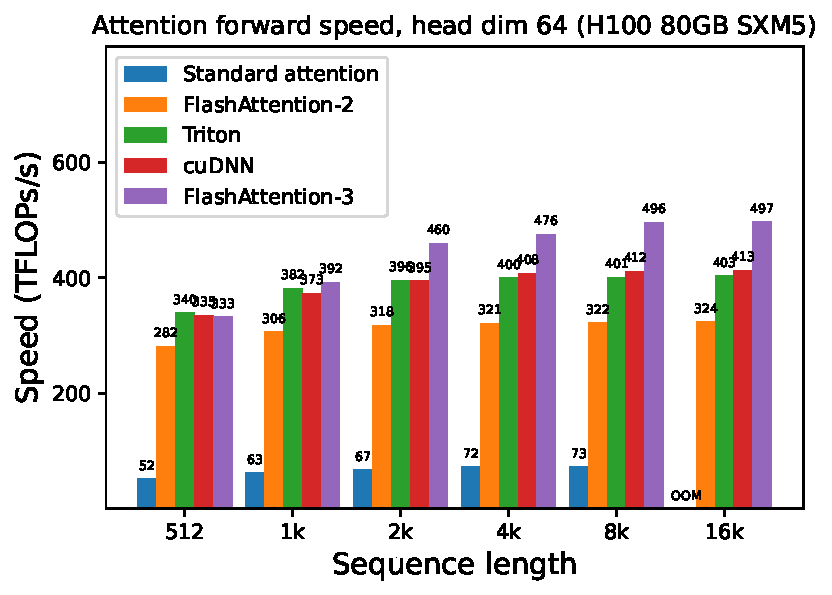
\includegraphics[width=.95\linewidth]{figs/flash3_h100_causal_False_hdim_64_fwd_speed.pdf}
    \caption{Forward, without causal mask, head dim 64}
  \end{subfigure}%
  \begin{subfigure}{.5\textwidth}
    \centering
    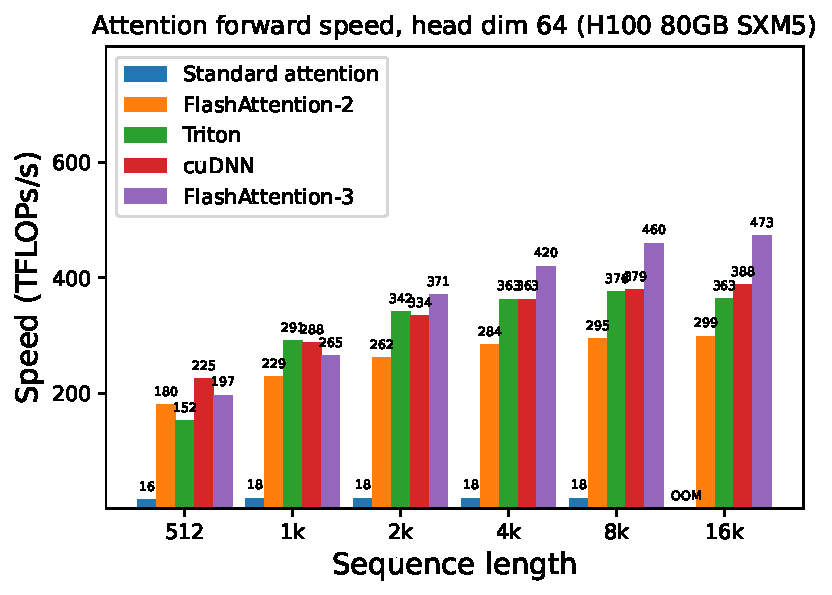
\includegraphics[width=.95\linewidth]{figs/flash3_h100_causal_True_hdim_64_fwd_speed.pdf}
    \caption{Forward, with causal mask, head dim 64}
  \end{subfigure}
  \begin{subfigure}{.5\textwidth}
    \centering
    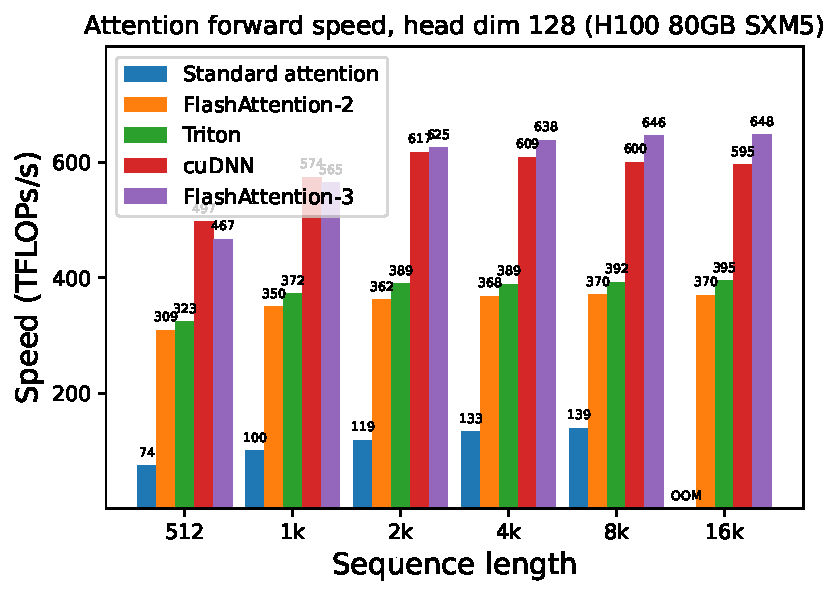
\includegraphics[width=.95\linewidth]{figs/flash3_h100_causal_False_hdim_128_fwd_speed.pdf}
    \caption{Forward, without causal mask, head dim 128}
  \end{subfigure}%
  \begin{subfigure}{.5\textwidth}
    \centering
    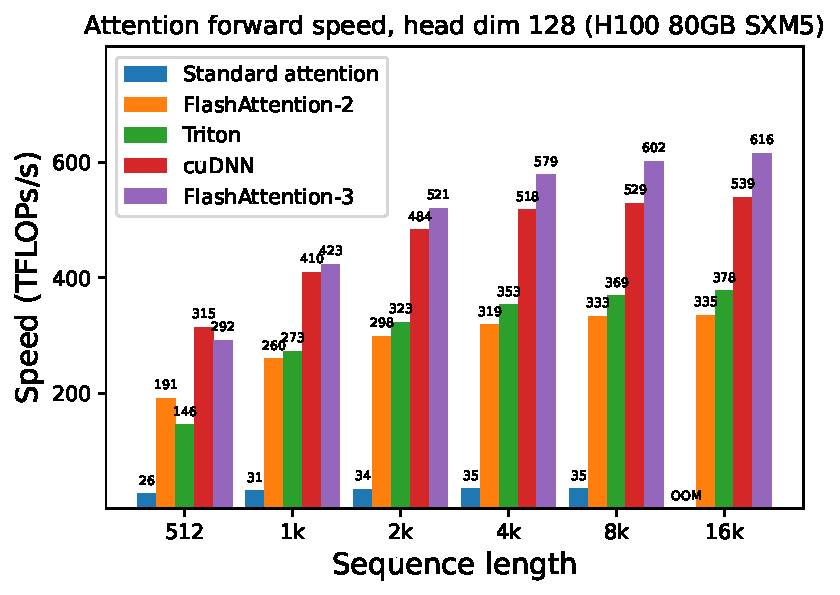
\includegraphics[width=.95\linewidth]{figs/flash3_h100_causal_True_hdim_128_fwd_speed.pdf}
    \caption{Forward, with causal mask, head dim 128}
  \end{subfigure}
  \begin{subfigure}{.5\textwidth}
    \centering
    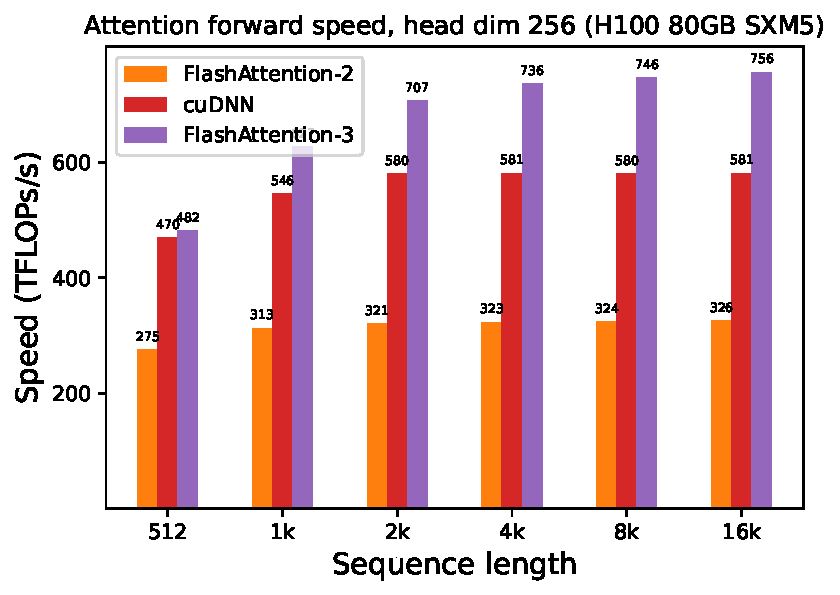
\includegraphics[width=.95\linewidth]{figs/flash3_h100_causal_False_hdim_256_fwd_speed.pdf}
    \caption{Forward, without causal mask, head dim 256}
  \end{subfigure}%
  \begin{subfigure}{.5\textwidth}
    \centering
    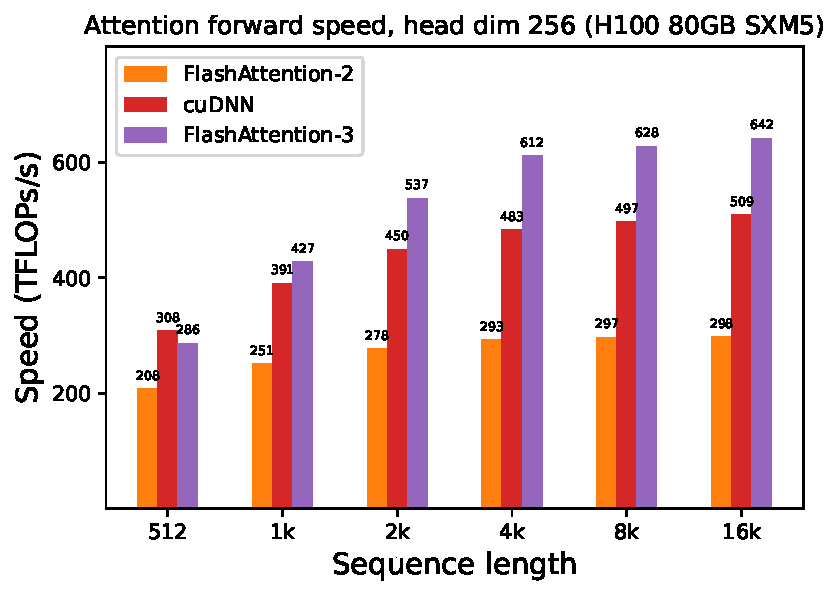
\includegraphics[width=.95\linewidth]{figs/flash3_h100_causal_True_hdim_256_fwd_speed.pdf}
    \caption{Forward, with causal mask, head dim 256}
  \end{subfigure}
  \caption{Attention forward speed (FP16/BF16) on H100 GPU}
  \label{fig:benchmark_attn_fwd}
\end{figure}

\begin{figure}[ht]
  \centering
  \begin{subfigure}{.5\textwidth}
    \centering
    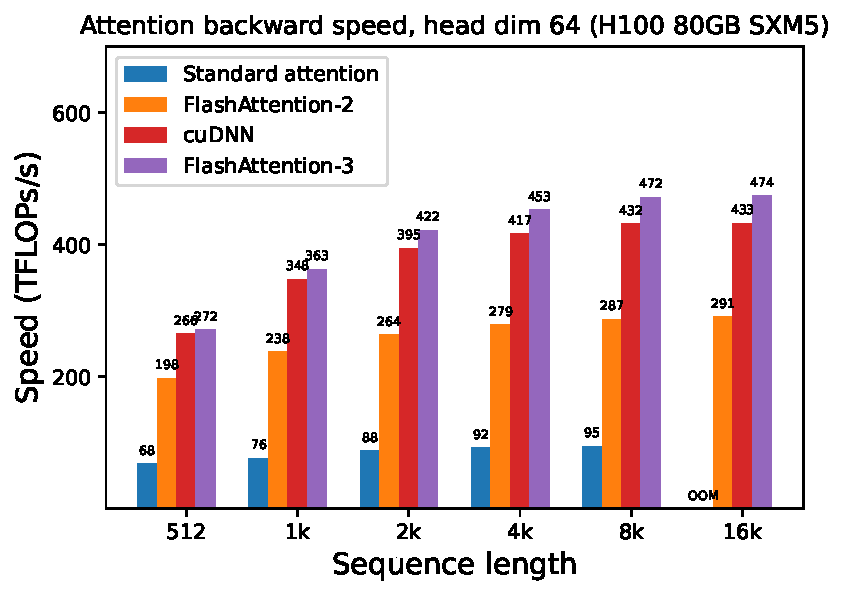
\includegraphics[width=.95\linewidth]{figs/flash3_h100_causal_False_hdim_64_bwd_speed.pdf}
    \caption{Backward, without causal mask, head dim 64}
  \end{subfigure}%
  \begin{subfigure}{.5\textwidth}
    \centering
    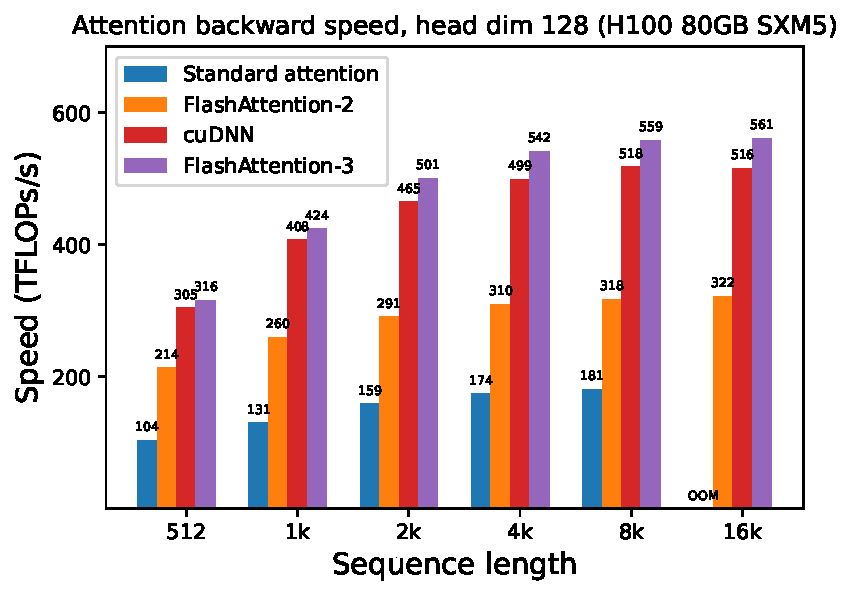
\includegraphics[width=.95\linewidth]{figs/flash3_h100_causal_False_hdim_128_bwd_speed.pdf}
    \caption{Backward, without causal mask, head dim 128}
  \end{subfigure}
  \caption{Attention backward speed (FP16/BF16) on H100 GPU}
  \label{fig:benchmark_attn_bwd}

\end{figure}

We also measure the runtime for FP8 for the forward pass under similar settings.
We report the results for headdim 256 in ~\cref{fig:benchmark_attn_fp8} and give the full results in \cref{sec:benchmark_attn_fp8_full}.

\begin{figure}[ht]
  \centering
  \begin{subfigure}{.5\textwidth}
    \centering
    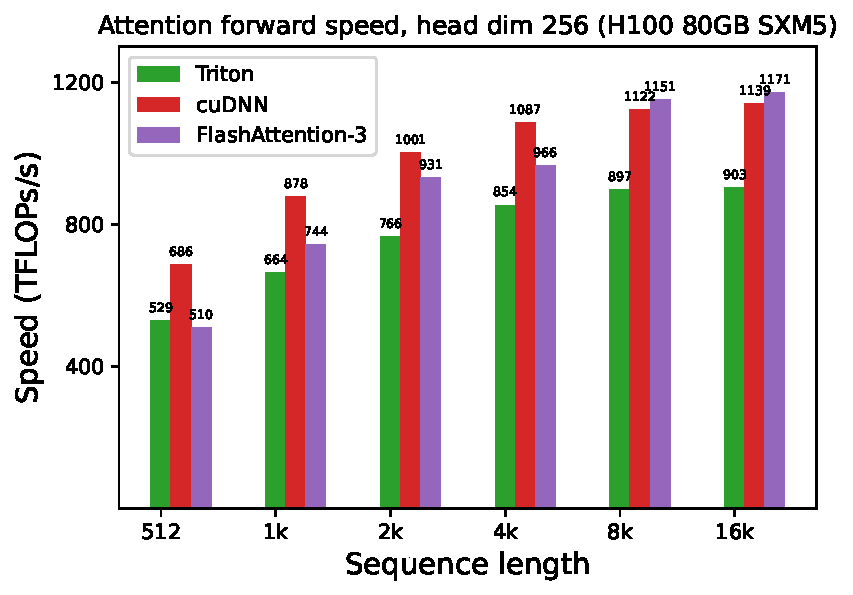
\includegraphics[width=.95\linewidth]{figs/flash3_h100_fp8_causal_False_hdim_256_fwd_speed.pdf}
    \caption{Forward, without causal mask, head dim 256}
  \end{subfigure}%
  \begin{subfigure}{.5\textwidth}
    \centering
    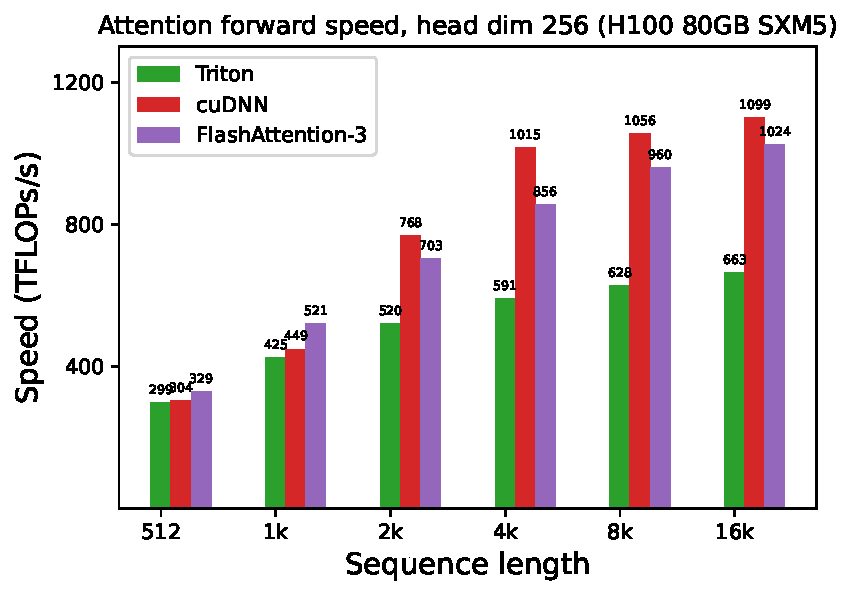
\includegraphics[width=.95\linewidth]{figs/flash3_h100_fp8_causal_True_hdim_256_fwd_speed.pdf}
    \caption{Forward, with causal mask, head dim 256}
  \end{subfigure}
  \caption{Attention forward speed (FP8) on H100 GPU}
  \label{fig:benchmark_attn_fp8}
\end{figure}

\subsection{Ablation Study: 2-Stage Pipelining Experiments}
\label{sec:2-stage-pipelining-experiments}

We ablate both the 2-stage WGMMA-softmax pipelining and warp-specialization for non-causal FP16 \fat with fixed parameters $\{\text{batch}, \text{seqlen}, \text{nheads}, \text{hdim}\} = \{ 4, 8448, 16, 128\}$.
The result in~\cref{table:ablation_pipelining} confirms that our algorithmic improvements (asynchrony with warp-specialization and overlapping between GEMM and softmax) lead to significant speedup, from 570 to 661 TFLOPs.
\begin{table}[h!]
  \centering  
  \caption{Pipelining ablation measurements}
  \label{table:ablation_pipelining}
  \begin{tabular}{|l|l|l|}
      \hline
      \textbf{Configuration} & \textbf{Time} & \textbf{TFLOPs/s} \\
      \hline
      \fat & 3.538 ms & 661 \\
      \hline
      No GEMM-Softmax Pipelining, Warp-Specialization & 4.021 ms & 582 \\
      \hline
      GEMM-Softmax Pipelining, No Warp-Specialization & 4.105 ms & 570 \\
      \hline
  \end{tabular}


\end{table}

\subsection{Numerical Error Validation}
\label{sec:numerical_error}

As there has been interest in the numerical error~\citep{golden2024flash} of
\fa, we compare \faa, \fat, and a standard implementation of attention against a
reference implementation in FP64.
To simulate outlier features and activations in LLMs~\citep{dettmers2208llm,
  sun2024massive}, we generate the entries of $\vQ, \vK, \vV$ with the following
distribution:
\begin{equation*}
  \mathcal{N}(0, 1) + \mathcal{N}(0, 100) \cdot \mathrm{Bernoulli}(0.001).
\end{equation*}
That is, each entry is normally distributed with zero mean and standard
deviation 1, but for 0.1\% of entries we add an independent term that's normally distributed
with standard deviation 10.
We then measure the root mean squared error (RMSE) in~\cref{table:numerical_error}.
In FP16, both \faa and \fat achieves 1.7$\times$ lower RMSE compared to the standard implementation since intermediate results (softmax) are kept in FP32.
The baseline attention in FP8 uses per-tensor scaling, with matmul accumulator in FP32 and intermediate softmax results kept in FP16.
Thanks to block quantization and incoherent processing, \fat in FP8 is 2.6$\times$ more accurate than this baseline.
\begin{table}[h!]
  \centering
  \caption{Numerical error comparisons in FP16 and FP8 (e4m3).}
  \label{table:numerical_error}
  \begin{tabular}{|c|ccc|}
      \hline
      Method & Baseline FP16 & \faa FP16 & \fat FP16 \\
      RMSE & 3.2e-4 & \textbf{1.9e-4} & \textbf{1.9e-4} \\
      \hline
  \end{tabular}
  \vspace{1em}
  \begin{tabular}{|c|cccc|}
      \hline
      Method & Baseline FP8 & \fat FP8 & No block quant & No incoherent processing \\
      RMSE & 2.4e-2 & \textbf{9.1e-3} & 9.3e-3 & 2.4e-2 \\
      \hline
  \end{tabular}
\end{table}
